\begin{figure}[p]
\centering
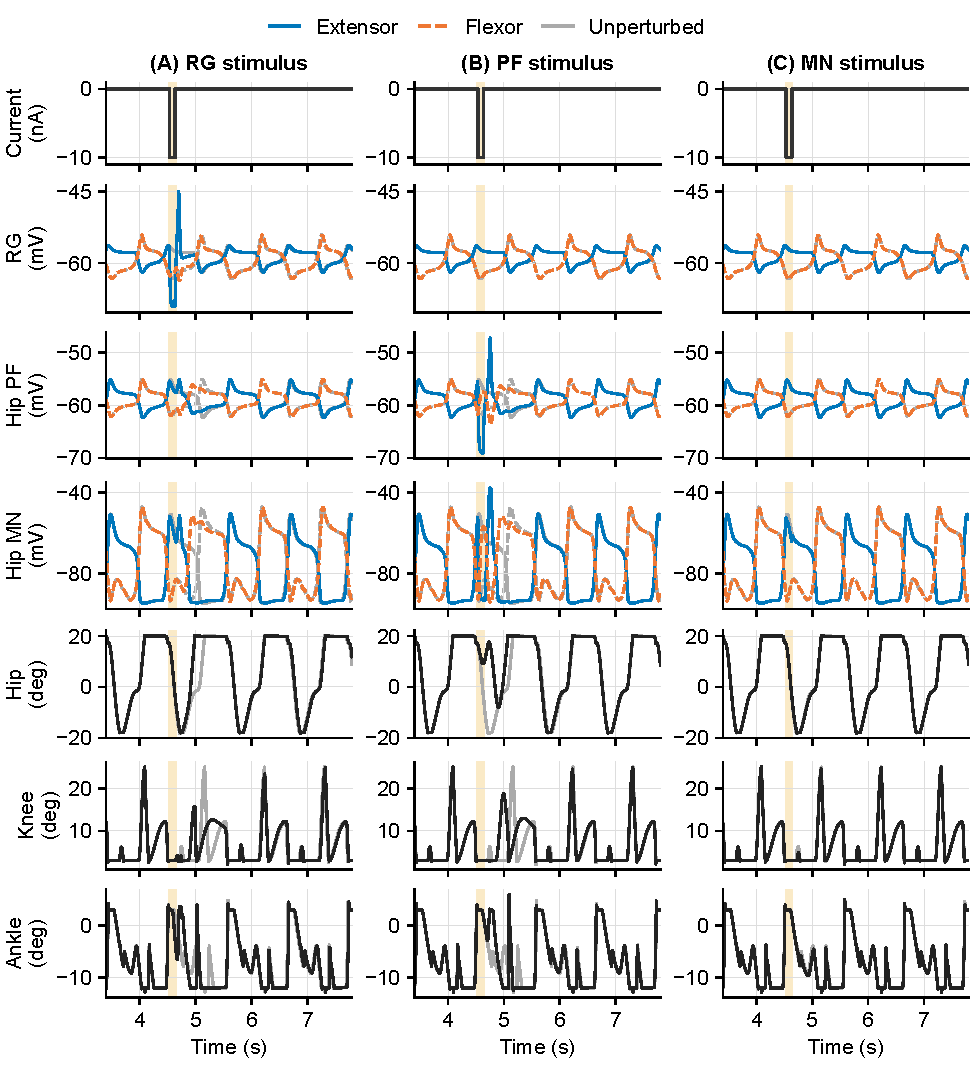
\includegraphics[width=\textwidth]{W2L108_left_RG_PF_MN_stimuli.pdf}
\caption[Layer-specific stimulation in the bilateral W2L controller]{Left-leg responses to separate extensor RG (A), hip PF (B), and hip MN (C) stimuli in the suspended W2L model. Each pulse is \qty{-10}{\nano\ampere} for \qty{100}{\milli\second}, beginning at \qty{4.534}{\second}; the top row shows the actual applied current, and shading marks its duration. Blue solid and orange dashed traces identify the named extensor and flexor neural pathways. Gray traces show the same neurons and joint angles without the test pulse; their solid and dashed neural traces retain the antagonist identities. Joint responses are black. The three columns use identical row scales and time limits. Neural voltages are recorded graded membrane potentials; joint angles retain the source anatomical convention, including positive knee flexion.}
\label{fig:w2l108_layer_stimuli}
\end{figure}

\begin{figure}[p]
\centering
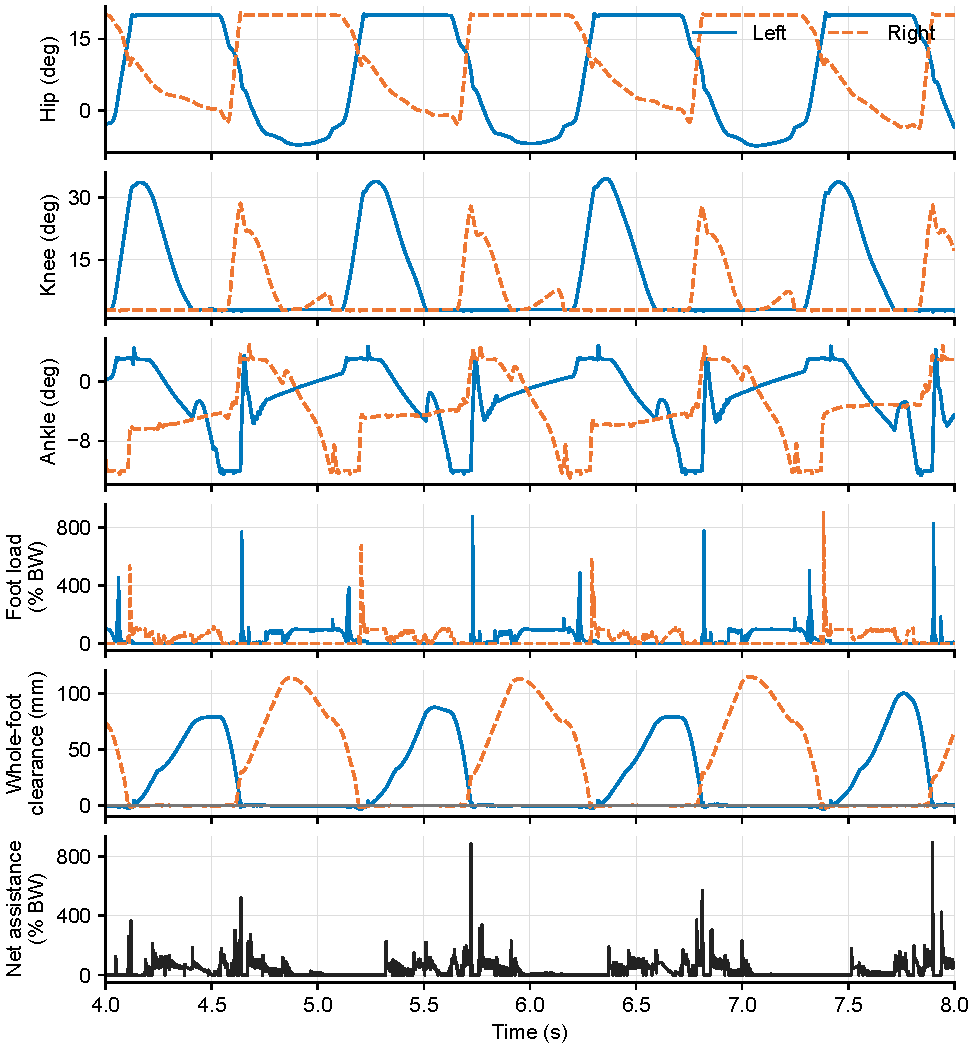
\includegraphics[width=\textwidth]{W2L108_tuned_ground_motion_load.pdf}
\caption[Supported stepping after W2L pose, phase, and gain corrections]{Joint motion, vertical foot load, minimum whole-foot clearance, and measured net vertical assistance in the fitted bilateral W2L configuration. Blue solid and orange dashed curves identify the left and right legs. The support apparatus consists of passive rails and a sliding guide with \qty{30}{\milli\meter} clearance. Assistance is the signed sum of measured rail, guide, and harness vertical reactions, divided by model body weight; the harness contribution is zero in this trial. The displayed interval retains the impact transients. Acceptance and assistance values in Table~\ref{tab:w2l108_ground_changes} are calculated over their stated scoring intervals rather than this plotted subset.}
\label{fig:w2l108_ground}
\end{figure}
